\documentclass[tikz,border=6pt]{standalone}
\usetikzlibrary{arrows.meta,calc}

\begin{document}
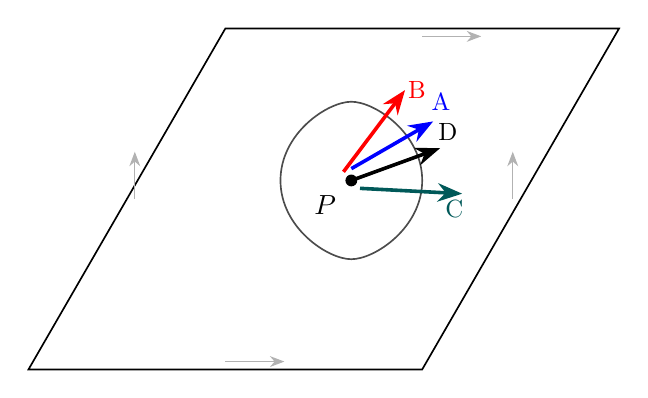
\begin{tikzpicture}[scale=5,>=Stealth]

% ---------- Lattice / fundamental domain (rhombus with 60° basis) ----------
\coordinate (A) at (0,0);
\coordinate (B) at (1,0);
\coordinate (C) at (1.5,0.866);
\coordinate (D) at (0.5,0.866);

% Central fundamental domain
\draw[line width=0.6pt,black] (A)--(B)--(C)--(D)--cycle;

% Edge-identification arrows
\draw[->,line width=0.5pt,gray!60] ($(A)!0.5!(B)$)++(0,0.02) -- ++(0.15,0);     % bottom: →
\draw[->,line width=0.5pt,gray!60] ($(D)!0.5!(C)$)++(0,-0.02) -- ++(0.15,0);    % top:    → (fixed)
\draw[->,line width=0.5pt,gray!60] ($(A)!0.5!(D)$)++(0.02,0) -- ++(0,0.12);     % left:   ↑
\draw[->,line width=0.5pt,gray!60] ($(B)!0.5!(C)$)++(-0.02,0) -- ++(0,0.12);    % right:  ↑ (fixed)

% ---------- Base point and loop ----------
\coordinate (P) at (0.82,0.48);
\fill (P) circle (0.015);
\node[below left=2pt] at (P) {$P$};

\draw[line width=0.6pt,black!70]
  ($(P)+(-0.18,0)$) .. controls ($(P)+(-0.18,0.12)$) and ($(P)+(-0.06,0.20)$) ..
  ($(P)+(0,0.20)$) .. controls ($(P)+(0.06,0.20)$) and ($(P)+(0.18,0.12)$) ..
  ($(P)+(0.18,0)$) .. controls ($(P)+(0.18,-0.12)$) and ($(P)+(0.06,-0.20)$) ..
  ($(P)+(0,-0.20)$) .. controls ($(P)+(-0.06,-0.20)$) and ($(P)+(-0.18,-0.12)$) ..
  cycle;

% ---------- Initial vector at P (rotated slightly clockwise) ----------
\def\ang{25}    % base direction (degrees)
\def\L{0.16}    % initial vector length
%\draw[->,line width=1.6pt,black] (P) -- ++({\ang-5}:\L);

% ---------- Candidate transported vectors (A, B, C unchanged) ----------
% (keep A, B, C blocks as they are)

% D: identical to the initial black arrow, rotated the same way, longer
\draw[->,line width=1.3pt,black]
  (P) -- ++({\ang-5}:0.24);
\node[black,scale=0.9] at ($(P)+({\ang-5}:0.24)+(0.02,0.04)$) {D};

% ---------- Candidate transported vectors (spread apart) ----------
% A: near the same direction, start slightly above P, modest length, rotated CCW
\draw[->,line width=1.3pt,blue]
  ($(P)+(0,0.030)$) -- ++({\ang+5}:0.24);
\node[blue,scale=0.9] at 
  ($(P)+(0,0.030)+({\ang+5}:0.24)+(0.02,0.05)$) {A};

% B: larger positive angle offset, start slightly left/up to separate tail
\draw[->,line width=1.3pt,red]
  ($(P)+(-0.020,0.022)$) -- ++({\ang+28}:0.26);
\node[red,scale=0.9] at ($(P)+(-0.020,0.022)+({\ang+28}:0.26)+(0.03,0.00)$) {B};

% C: larger negative angle offset, start slightly right/down to separate tail
\draw[->,line width=1.3pt,teal!70!black]
  ($(P)+(0.022,-0.020)$) -- ++({\ang-28}:0.26);
\node[teal!70!black,scale=0.9] at ($(P)+(0.022,-0.020)+({\ang-28}:0.26)+(-0.02,-0.04)$) {C};



\end{tikzpicture}
\end{document}